\section{Bài 3: Traceroute}
Nếu bạn dùng Window thì dùng lệnh \textbf{\textit{tracert}}, nếu bạn dùng Linux/iOS thì bạn dùng lệnh \textbf{\textit{traceroute}}. Lưu ý kết quả bắt gói tin trên Window và Linux/iOS sẽ khác nhau, vì vậy câu trả lời phụ thuộc bạn dùng OS nào.\\
Bật wireshark để bắt gói tin lệnh traceroute từ máy của mình (có thể dùng máy ảo) đến \textbf{\textit{www.fit.hcmus.edu.vn}} (FIT). \\
Bài tập được thực hiện trên máy tính sử dụng hệ điều hành \textbf{Windows 11}.\\
Kết quả bắt gói tin chi tiết được lưu trong tập tin \textbf{bai3.pcapng}.\\

\textbf{1. Chụp hình kết quả bắt gói tin sau khi traceroute hoặc tracert (thấy được những gói tin liên quan).}\\
Kết quả bắt gói tin sau khi tracert như sau.
\begin{figure}[H]
\begin{center}
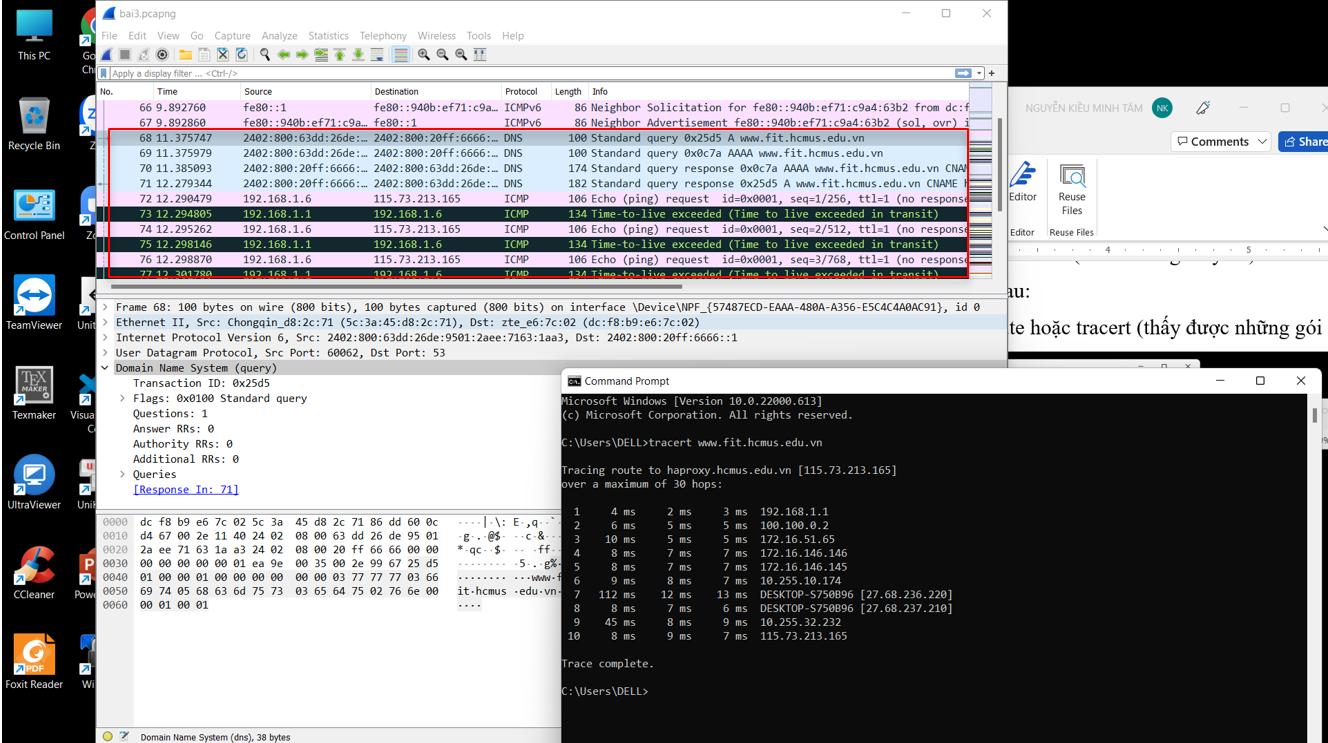
\includegraphics[scale=.8]{../figures/p3/p3_res1}
\end{center}
\caption{Kết quả bắt gói tin sau khi tracert}
\end{figure}
Các gói tin được bắt tính từ lệnh tracert được thể hiện ở phần đóng khung màu đỏ trên hình vẽ. Đó là các gói tin đầu tiên bắt đầu từ khi tracert (gói tin số 68).

\textbf{2. Cho biết traceroute/tracert dùng để làm gì?}\\
Traceroute/tracert dùng để xác định vết đường đi của gói tin giữa hai host: source host và destination host. 
Thông tin này được thể hiện qua các gói tin ICMP (gói tin IP có trường protocol = 1). Và dựa vào thông tin tương ứng trên các trường của thông điệp ICMP, host nguồn xác định được địa chỉ IP của các router trên đường truyền. \supercite{cn, slides}

\textbf{3.	Cho biết địa chỉ IP của máy gửi request.}\\
Địa chỉ IP của máy gửi request là 192.168.1.6.
\begin{figure}[H]
\begin{center}
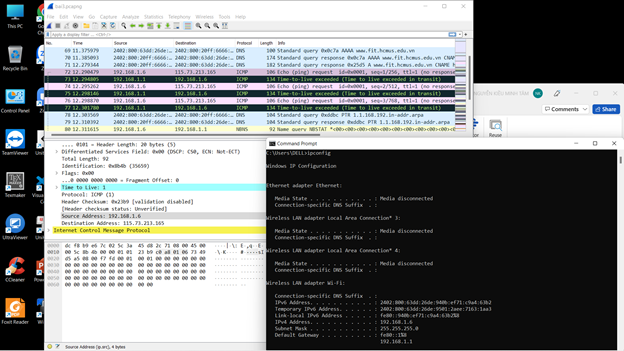
\includegraphics[scale=.8]{../figures/p3/p3_hostip}
\end{center}
\caption{Địa chỉ IP của máy gửi request}
\end{figure}

\textbf{4.	Cho biết cách máy tính xác định được địa chỉ IP của FIT.}\\
Máy tính sẽ gửi gói tin DNS query lên DNS server để “hỏi”, sau đó DNS Server sẽ trả lời qua gói tin DNS response. 
\begin{itemize}
\item Gói tin DNS query được gửi từ destination host là gói tin số 68 (được lưu trong file \textbf{bai3.pcapng}).
\begin{figure}[H]
\begin{center}
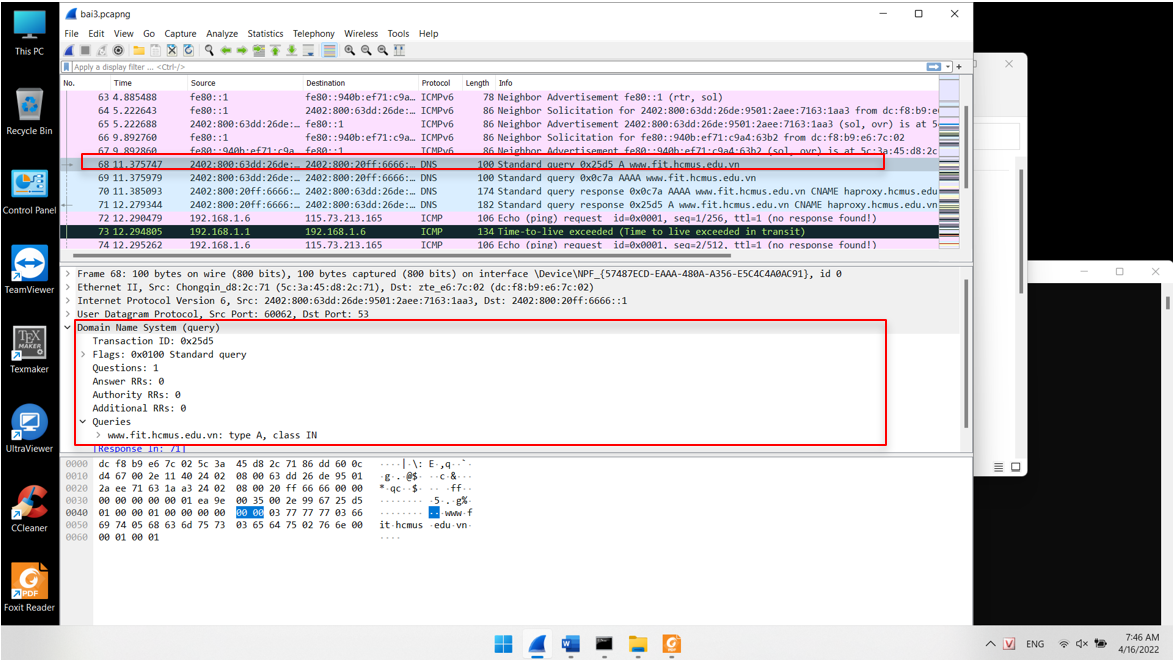
\includegraphics[scale=.8]{../figures/p3/p3_dns1}
\end{center}
\caption{Gói tin DNS query}
\end{figure}
\item Và gói tin trả lời tương ứng là gói tin số 71 (được lưu trong file \textbf{bai3.pcapng}). Hình vẽ cho thấy có FIT có 3 địa chỉ IP 115.73.213.165, 14.161.23.204, 14.241.254.131. Trong lần này traceroute được thực hiện tới địa chỉ IP 115.73.213.165. 
\begin{figure}[H]
\begin{center}
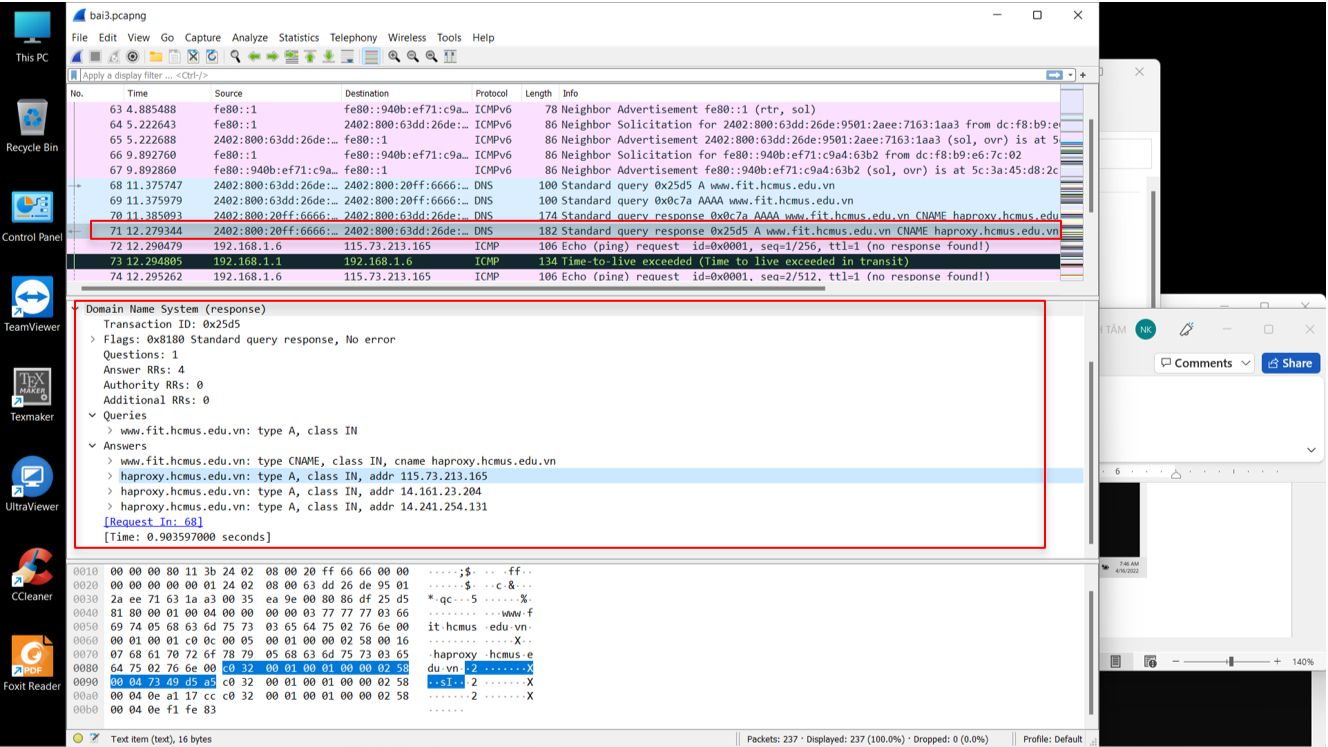
\includegraphics[scale=.8]{../figures/p3/p3_dns2}
\end{center}
\caption{Gói tin DNS query response}
\end{figure}
\end{itemize}

\textbf{5.	Sau khi xác định được IP của www.fit.hcmus.edu.vn, máy sẽ bắt đầu gửi gói tin đến FIT.}\\
\textbf{a.	Protocol được sử dụng của những gói tin sau đó là gì?}\\
Protocol được sử dụng trong những gói tin sau đó là ICMP, bắt đầu từ gói tin số 72 trong file \textbf{bai3.pcapng} (phần đóng khung màu đỏ trong hình \ref{fig351}).

\begin{figure}[H]
\begin{center}
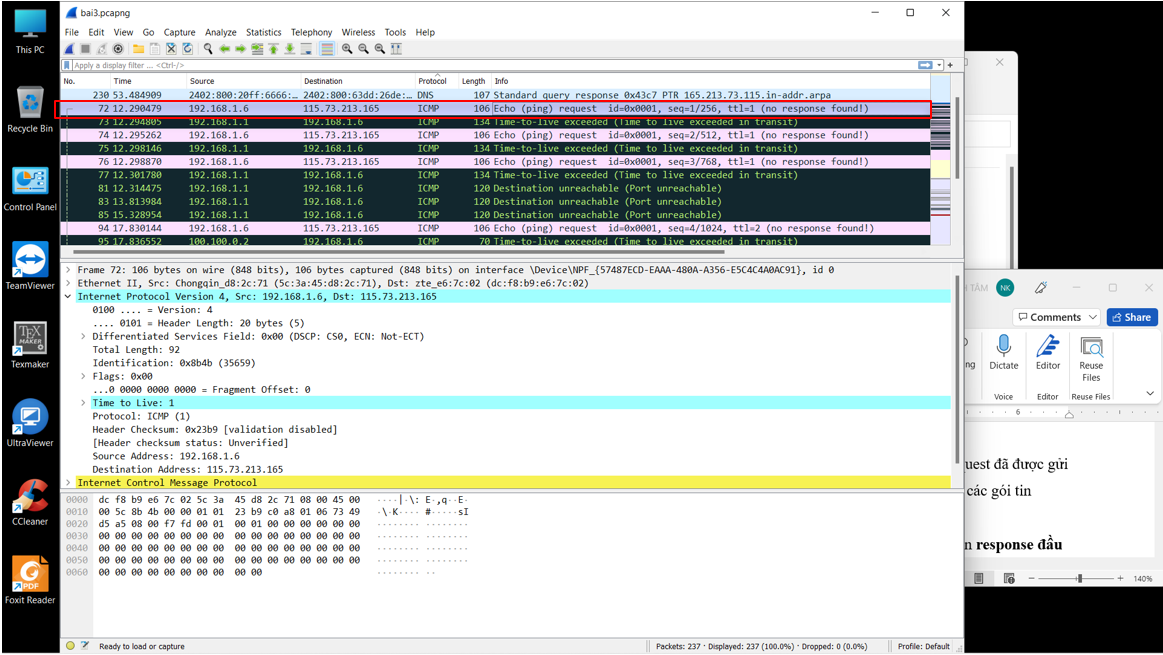
\includegraphics[scale=.8]{../figures/p3/p3_51}
\end{center}
\caption{Protocol được sử dụng}
\label{fig351}
\end{figure}

\textbf{b.	Có bao nhiêu gói tin được gửi đi (request) trước khi nhận được response đầu tiên trả lời cho những request? (Hay nói một cách khác là: lệnh trace* sẽ gửi request message đi, và nhận về response. Vậy có bao nhiêu gói tin request đã gửi đi đến khi nhận được gói tin response đầu tiên?)}\\
Tính từ gói tin request đầu tiên (gói tin số 72) có tổng cộng \textbf{28 gói tin} request đã được gửi trước khi nhận được respone message đầu tiên (gói tin số 224), không kể các gói tin không liên quan khác.

\textbf{c.	Cho biết TTL của gói tin cuối cùng được gửi trước khi nhận được gói tin response đầu tiên trả lời cho những gói tin request?}\\
TTL của gói tin cuối cùng được gửi trước khi nhận được gói tin response đầu tiên trả lời cho những gói tin request là 10 (gói tin 223, phần đóng khung màu vàng trong hình \ref{fig352}).
\begin{figure}[H]
\begin{center}
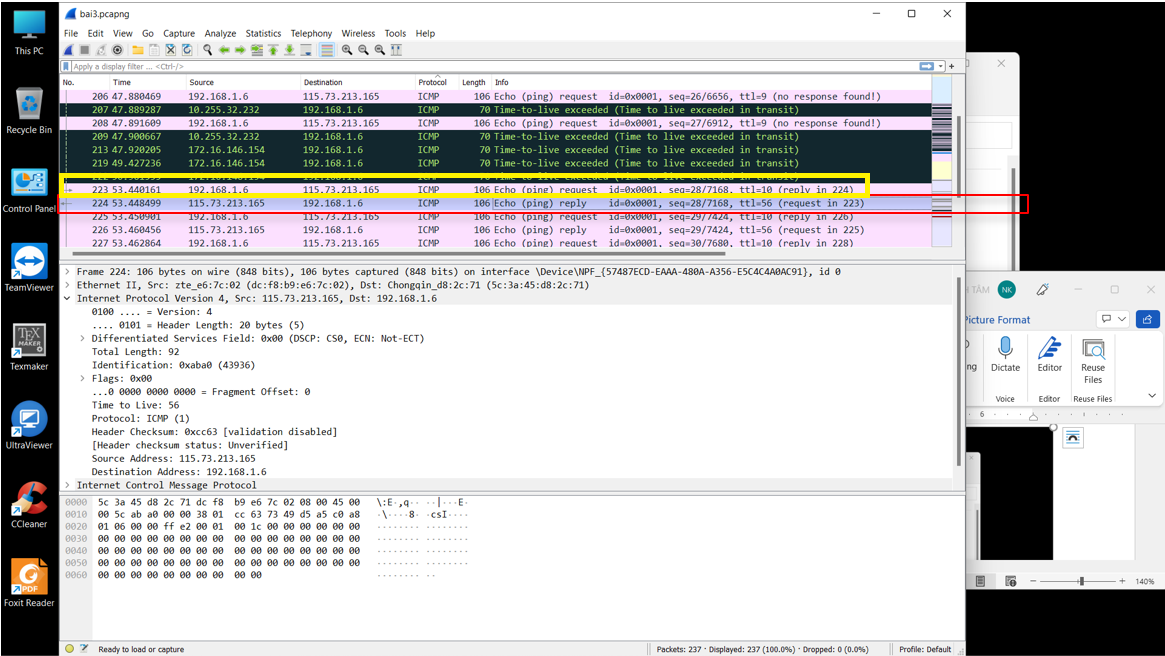
\includegraphics[scale=.8]{../figures/p3/p3_52}
\end{center}
\caption{TTL của gói tin cuối cùng trước khi nhận response}
\label{fig352}
\end{figure}

\textbf{d.	Bạn có thấy thông tin port trong các gói tin gửi đi? Nếu có bạn nhận thấy port nguồn/đích của gói tin có gì đặc biệt? Nếu không thấy thông tin port, hãy giải thích nguyên nhân.}\\
Trong các gói tin gửi đi không tìm thấy thông tin port. Vì nghi thức ICMP hoạt động ở tầng Network, trong khi số hiệu port là “địa chỉ” của ứng dụng, được sử dụng ở tầng Application.

\textbf{e.	Gói tin response đầu tiên là trả lời cho gói tin request thứ mấy? (No.)}\\
Gói tin response đầu tiên (gói tin số 224) trả lời cho gói tin request thứ 28 (gói tin số 223) (phần đóng khung màu đỏ trong hình \ref{fig352}).